\chapter{Causal Algorithmic Recourse} \label{chapter:causal_recourse}

In the introduction, three problems with cost functions used in the literature were outlined. The first of these was that actions are typically enacted sequentially (e.g., you first increase your income, and then increase your savings). This is important within the \textit{causal} algorithmic setting, where intervening on a variable (e.g, increasing income) has downstream (causal) effects on other variables such as savings. In this chapter, we first motivate \textit{causal} algorithmic recourse, then explore causal algorithmic recourse with soft, as opposed to hard interventions and finally propose a solution to optimise for ordering of sequential interventions when generating recourse.

\section{Motivation}

As discussed in section \ref{section:cost_functions_lit_review}, the cost of changing features is typically modelled as an $\cost(\mathbf{x,x}')=L_p(\mathbf{x} - \mathbf{x}')$ or the total log percentile shift \citep{ustunActionableRecourseLinear2019}. These cost functions fail to take into account the downstream (causal) effects of changing one feature on other features.\\

In order to correctly measure the cost of changing from features $\mathbf{x}$ to $\mathbf{x}'$, we need to be able to evaluate the causal effects of changing one variable on others. For example, if an individual decides not to inquire about a loan for a number of months (which will change the feature ``number of inquiries in the last 6 months'', the cost of decreasing the feature ``number of inquiries in the last 6 months, excluding the last 7 days'' will be very low or zero. However, if a quadratic cost function (or any $L_p$ norm cost function) is used, this will be interpreted as two separate feature changes and the costs of each will be summed. Whilst this simple case can likely be handled by domain expertise, more complex causal relations will exist. Consider an individual obtaining two more credit cards. Whilst this may reduce the cost of increasing ``number of credit cards'', this may also increase the cost of ``monthly credit card payments'' and may have less clear effects (which need not be linear) on other features.\\

The Mahalanobis distance cost function $\texttt{cost}(\mathbf{x}, \mathbf{x}') = (\mathbf{x} -\mathbf{x}')^T\mathbf{M}(\mathbf{x} - \mathbf{x}')$, where $\mathbf{M}$ is a fixed, known, positive semi-definite square matrix \citep{bechavodInformationDiscrepancyStrategic2022}, does allow for changing one feature to affect the cost of changing other features through the off-diagonal elements in $\mathbf{M}$ (see equation \ref{eq:mahalanobis_example} for a worked example). However, the causal effects rely on the changes being made simultaneously. If we first apply a change to $\mathbf{x}_1$ and then to $\mathbf{x}_2$, as shown below. In equations \ref{eq:mahalanobis_step1} and \ref{eq:mahalanobis_step2}, the changes are applied sequentially and there are no causal effects, leading to a total cost of 5. In equation \ref{eq:mahalanobis_step3}, the changes are applied simultaneously and the effect of changing $\mathbf{x}_1$ leads a lower cost of changing $\mathbf{x}_2$, with a total cost of 4. The importance of sequential changes as opposed to simultaneous changes are discussed in section \ref{section:soft_interventions}.

\begin{equation} \label{eq:mahalanobis_step1}
	[1, 0, 0]^T \left[\begin{array}{lllll}
		1 & 0 & 0 \\
		-0.5 & 1 & 0 \\
		0 & 0 & 1
	\end{array}\right] [1, 0, 0]^T = 1^2 + 0^2 + 0^2 = 1
\end{equation}

\begin{equation} \label{eq:mahalanobis_step2}
	[0, 2, 0]^T \left[\begin{array}{lllll}
		1 & 0 & 0 \\
		-0.5 & 1 & 0 \\
		0 & 0 & 1
	\end{array}\right] [0, 2, 0]^T = 0^2 + 2^2 + 0^2 = 4
\end{equation}

\begin{equation} \label{eq:mahalanobis_step3}
	[1, 2, 0]^T \left[\begin{array}{lllll}
		1 & 0 & 0 \\
		-0.5 & 1 & 0 \\
		0 & 0 & 1
	\end{array}\right] [1, 2, 0]^T = 1^2 + 1.5(2) + 0^2 = 4
\end{equation}


\section{Structural Causal Models} \label{section:scms}

To incorporate changing one feature having a causal effect on the cost of changing another feature, we must model the effect of changing the feature $\mathbf{x}_1$ to $\mathbf{x'}_1$ has on changing the feature $\mathbf{x}_2$ to $\mathbf{x'}_2$. Following \textcite{karimiAlgorithmicRecourseCounterfactual2021}, we can model the world using a structural causal model (SCM) to account for downstream effects. The SCM can be defined formally as $\mathcal{M} = \langle\mathbb{U, V, F}\rangle$ capture all the causal relations in the world, where $\mathbb{U}$ represents set of exogenous variables, $\mathbb{V}$ represents the set of endogenous variables (all are a descendant of at least one of the variables in $\mathbb{U}$) and $\mathbb{F}$ represents the set of structural equations which describe how the endogenous variables can be determined from the exogenous variables \citep{pearl2016causal}.

We can illustrate a simple SCM $\mathcal{M}$ with $\mathbb{U} = \{x_1\}$, $\mathbb{V} = \{x_2, x_3, x_4\}$ and structural equations $\mathbb{F}$ are defined in equation \ref{eq:toy_structural_equations}.

\begin{align} \label{eq:toy_structural_equations}
	x_1 & = u_1 & u_1 \sim N(30 , 5) \\ \nonumber %income
	x_2 & = u_2 + 0.5x_1 & u_2 \sim N(20, 10) \\ \nonumber %savings
	x_3 & = u_3 - 0.25x_2 & u_3 \sim \text{Uniform}(0, 20) \\ \nonumber %debt
	x_4 & = \frac{x_3}{x_1} %debt to income ratio
\end{align}


\begin{figure}[!htb]
	\centering
	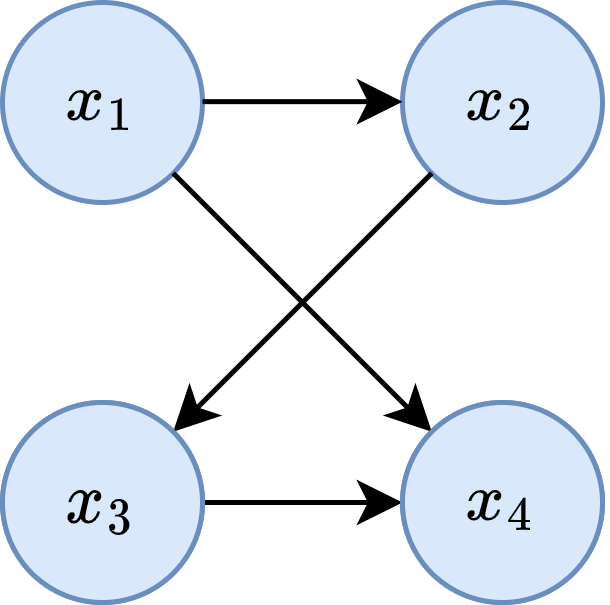
\includegraphics[width=0.25\linewidth]{images/draw.io/Simple SCM.png}
	\caption{Causal graph $\mathcal{G}$ of SCM $\mathcal{M}$.}
	\label{fig:toy_scm}
\end{figure}


The SCM can also be presented with a causal graph $\mathcal{G}$, which is shown in Figure \ref{fig:toy_scm}. Let $x_1$ represent salary (in thousands of pounds), $x_2$ represent savings (in thousands of pounds), $x_3$ represent the debt (in thousands of pounds) and $x_4$ represent debt-to-income ratio. If an individual for whom the SCM $\mathcal{M}$ holds receives an increase in salary, this will lead to an increase in savings and a reduction the debt-to-income ratio. If the individual's initial features were [£30,000, £25,000, £10,000, 1/3]$^T$ and their salary increases to £35,000, then it should then be easier to increase their savings and decrease their debt-to-income ratio than when their salary was £30,000. This toy example shows how the SCM $\mathcal{M}$ encodes the downstream effect of increased salary on both savings and probability of mortgage approval.

[\textbf{DISCUSSION ON PEARL-STYLE DAGS/INBENS CRITIQUE}]

We can use the Abduction-Action-Prediction steps \citep{pearl2016causal} to obtain a \textit{structural counterfactual} of an increase in salary ($x_1$) from £30,000 to £35,000, given that the existing features are [£30,000, £25,000, £10,000, 1/3]$^T$ \comment{go over this example again, should be such that the hard intervention actually leads to the severing of an edge to illustrate the point on hard interventions}

\textbf{1. Abduction}. Calculate the value of exogenous variables before intervention, given the evidence (the current values of the features).

\begin{align}
	u_1 & = x_1 & =  30,000 \\ \nonumber
	u_2 & = x_2 - 0.5x_1 = 25,000 - 0.5(30,00) & = 10,000 \\ \nonumber
	u_3 & = x_3 + 0.25x_2 = 10,000 + 0.25(25,000) & = 16,250
\end{align}

\textbf{2. Action}. Modify the model $\mathcal{M}$ by implementing the intervention on $x_1$ (i.e\., $do(x_2=30,000)$). This leads to a new SCM $\mathcal{M}_1$ where all incoming edges to the intervened upon variable $x_2$ are severed and the value of the intervened upon variable $x_2$ is set to the intervention value £30,000. The resulting SCM $\mathcal{M}_1$ is shown in Figure \ref{fig:toy_scm_severed}, with structural equations $\mathcal{F}_1$.

\begin{figure}[!htb]
	\centering
	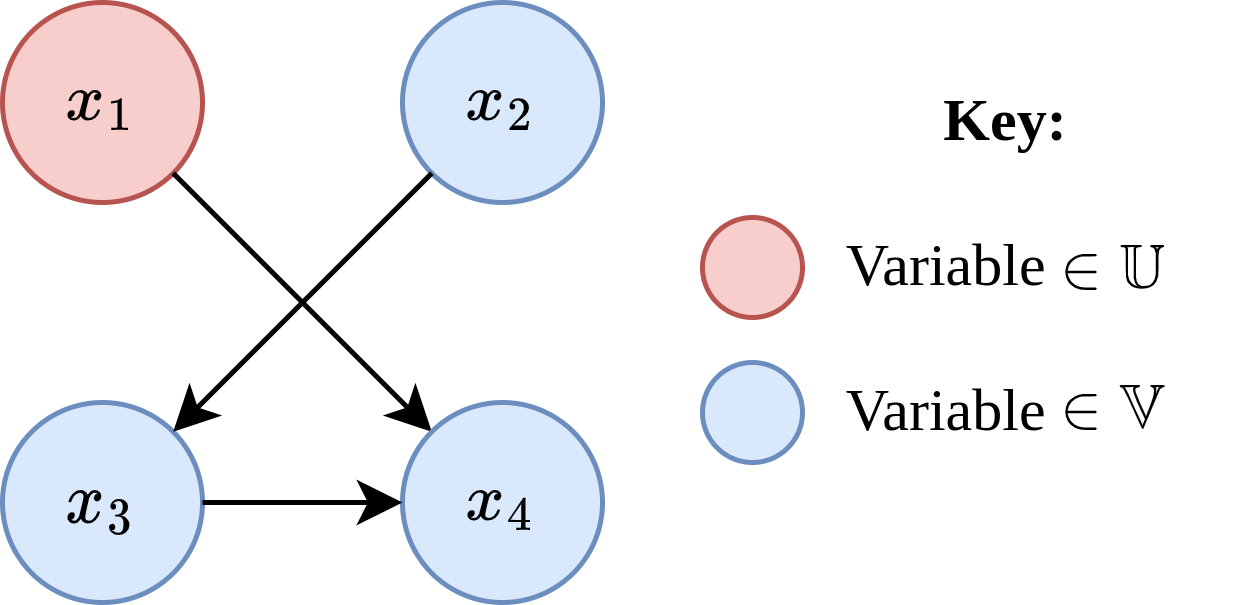
\includegraphics[width=0.25\linewidth]{images/draw.io/Simple SCM Severed.png}
	\caption{Causal graph $\mathcal{G}$ of SCM $\mathcal{M}_1$.}
	\label{fig:toy_scm_severed}
\end{figure}

\begin{align}
	x_1 & = u_1 \\ \nonumber
	x_2 & = 30,000 \\ \nonumber
	x_3 & = u_3 - 0.25x_2 \\ \nonumber %debt
	x_4 & = \frac{x_3}{x_1} %debt to income ratio
\end{align}

\textbf{3. Prediction}. Using the updated model $\mathcal{M}_1$ and values of exogenous variables $\mathbf{u}$, calculate the values of the endogenous variables.

\begin{align}
	x^{\text{SCF}}_1 & = u_1 &  = 30,000 \\ \nonumber
	x^{\text{SCF}}_2 & = 30,000 & = 30,000 \\ \nonumber
	x^{\text{SCF}}_3 & = u_3 - 0.25x^{\text{SCF}}_2 = 16,250 - 0.25(30,000) & = 8,750 \\ \nonumber
	x^{\text{SCF}}_4 & = \frac{x^{\text{SCF}}_3}{x^{\text{SCF}}_1} = \frac{8,750}{30,000} & = 0.292
\end{align}

Mathematically, we can denote the Action-Abduction-Prediction steps as shown in equation \ref{eq:hard_intervention}, where $I$ is the set of indices of intervened on variables, $\delta_i$ is the action on variable $i$, $f_i \in \mathbb{F}$ is structural equation of the variable $i$,  $\text{pa}_i$ are the parents of variable $i$, $I$ is the set of variables that intervened upon (e.g, ) and $\mathbb{I}$ is the indicator function.

\begin{align} \label{eq:hard_intervention}
	x^{\text{SCF}}_i = & \mathbb{I}_{i \in I} (x_i + \delta_i) + \mathbb{I}_{i \notin I} \bigg(x_i + f_i(\text{pa}^{\text{SCF}}_i) - f_i(\text{pa}_i)\bigg)
\end{align}


To calculate recourse $\mathbf{x}^*$ with an SCM over all the features within $\mathbf{x}$, we need to re-formulate the original algorithmic recourse optimisation problem presented in equation \ref{eq:recourse_setup}. Following \textcite{karimiAlgorithmicRecourseCounterfactual2021}, we replace the minimising the cost of changing features from $\mathbf{x}$ to $\mathbf{x}'$ with minimising the cost of \textit{interventions} $A = \text{do} \{\mathbf{x}_i:=\mathbf{x}_i + \boldsymbol{\delta}_i\}_{i=1, \ldots, D}$ where $D$ is the number of features. The updated recourse problem is shown in equation \ref{eq:causal_recourse_problem_hard}.

\begin{align} \label{eq:causal_recourse_problem_hard}
	A^* = & \argmin_{A} \texttt{cost}(\mathbf{x}, A) \\ \nonumber
	\text{s.t. } & h(\mathbf{x}^{\text{SCF}}) = 1, \\ \nonumber
	& \mathbf{x}^{\text{SCF}}_i = \mathbb{I}_{i \in I} (\mathbf{x}_i + \boldsymbol{\delta}_i) + \mathbb{I}_{i \notin I} \bigg(x_i + f_i(\textbf{pa}^{\text{SCF}}_i) - f_i(\textbf{pa}_i)\bigg), \\ \nonumber
	& A \in \mathcal{F}
\end{align}

We define the cost of interventions $A$ on original features $\mathbf{x}$ as the sum of the cost of the individual actions. The cost of each individual action is left to be flexible, and can represent a variety of cost functions, such as the $L_p$-norm of $\boldsymbol{\delta}_i$ or a percentile shift based cost function such as that used by \textcite{ustunActionableRecourseLinear2019}.

\begin{equation}
	\texttt{cost}(\mathbf{x}, A) = \sum_{i=1}^{D} c \bigg(\text{do}(\mathbf{x}_i:=\mathbf{x}_i + \boldsymbol{\delta}_i) \bigg)
\end{equation}

This formulation relies on two key assumptions.

\textbf{Assumption 1}. The interventions are structural (hard) interventions, where after intervening on a variable, all incoming edges to its corresponding node in the causal graph are severed. If an individual were to intervene on savings ($x_2$) (perhaps by selling their car or borrowing from family), then we assume that they then stop saving a proportion of their income (severing the edge between $x_1$ and $x_2$).

\textbf{Assumption 2}. Interventions on multiple variables are carried out simultaneously. Given an intervention A = [£32,000, £27,500, £10,000, 1/3]$^T$, it is assumed that salary as increased at the same time as savings, as opposed to taking place sequentially.

\subsection{Soft (Parametric) Interventions} \label{section:soft_interventions}

In many cases where recourse is provided, such as credit scoring, it is unlikely that intervening on a variable leads to all incoming edges to its corresponding node in the causal graph being severed - a violation of assumption 1. Intervening on savings is unlikely to lead to an individual stopping saving their salary. Likewise, intervening on body fat levels through liposuction does not lead to diet having no causal effect on body fat levels. Structural (hard) interventions are typically used in randomised control trials. For example, in a medical trial, patients are assigned to either to receive either a treatment or a placebo. Any other variables that may have caused the patient to receive a treatment or not now have no causal effect, as in carrying out the trial we simply assign the patient to receive either the treatment or a placebo.

In the cases where assumption 1 is violated, we can then represent the interventions as soft (or parametric) interventions, which do not result in severing of incoming edges \citep{eberhardtInterventionsCausalInference2007}. After the soft (parametric) intervention, we denote the resulting value of $\mathbf{x}$ after the intervention as $\mathbf{x}^{\text{PCF}}$, the \textit{parametric} counterfactual, which is defined below.

\begin{equation} \label{eq:soft_interventions}
	x^{\text{PCF}}_i = \mathbb{I}_{i \in I} \delta_i + \bigg( x_i + f_i(\text{pa}^{\text{PCF}}_i) - f_i(\text{pa}_i) \bigg)
\end{equation}

As the majority of interventions which take place in the context of algorithmic recourse, such as increasing savings and re-taking an test such as the GMAT/GRE (in the case of recourse for postgraduate admissions) do not tend to result in the severing of incoming edges such as the proportion of income saved and the effect of additional revision on test scores, soft interventions are implemented in this thesis. Using soft interventions results in an updated causal recourse problem shown below in equation \ref{eq:causal_recourse_problem_soft}.

\begin{align} \label{eq:causal_recourse_problem_soft}
	A^* = & \argmin_{A} \texttt{cost}(\mathbf{x}, A) \\ \nonumber
	\text{s.t. } & h(\mathbf{x}^{\text{PCF}}) = 1, \\ \nonumber
	& 	\mathbf{x}^{\text{PCF}} = \mathbb{I}_{i \in I} \boldsymbol{\delta}_i + \bigg( \mathbf{x}_i + f_i(\textbf{pa}^{\text{PCF}}_i) - f_i(\textbf{pa}_i) \bigg), \\ \nonumber
	& A \in \mathcal{F}
\end{align} 


\subsection{Sequential Interventions}

Assumption 2 of the causal recourse problem formulation in \ref{eq:hard_intervention} is that all interventions occur simultaneously. Picture a scenario where an individual is rejected from a PhD program, and the recourse interventions are to gain more research experience (potentially through a pre-doctoral fellowship or research assistant position) and obtain a more favourable letter of recommendation. In the real world, it is likely that these actions will be carried out sequentially, where research experience is obtained first and the letter of recommendation is second (as the professor for whom the applicant is conducting their research under will likely be the author of the letter of recommendation), as opposed to occurring simultaneously.

Using equation \ref{eq:soft_interventions}, the order of the intervention does not affect the counterfactual values\comment{Potentially worth showing how $f_i(\text{pa}^{\text{PCF}}_i)$ in one intervention is cancelled out by $f_i(\text{pa}_i)$ in the next intervention} $x^{\text{PCF}}_i$, but can affect the cost of actions $A$.


\begin{proposition} \label{sequential_proposition}
	In a sequential intervention setting with $n$ separate interventions where $x_i$ and $x_j$ are intervened upon, if the cost of individual interventions $c(\text{do}(x_i:=x_i + \delta_i))$ depends on the value of $x_i$ and $x_i$ is a descendent of $x_j$, then the ordering of the sequential interventions affects the total cost of the $n$ sequential interventions.
\end{proposition}

\begin{proof}
	The values of $x_i$ after an intervention on $x_i$ and intervening on $x_j$ are shown below.
	\begin{align} \label{eq:proposition_1_equation}
		x^{\text{PCF}_i}_i & = x_i + \delta_i \\ \label{eq:proposition_1_equation2}
		x^{\text{PCF}_j}_i & = x_i + f_i(\text{pa}^{\text{PCF}}_i) - f_i(\text{pa}_i)
	\end{align}
	As the cost of individual interventions depends on the value of $x_i$ before intervention, the cost of intervening on $x_i$ first depends on the value $x_i$ whereas the cost of intervening on $x_i$ second depends on the value $x_i + f_i(\text{pa}^{\text{PCF}}_i) - f_i(\text{pa}_i)$ (the value after intervening on $x_j$, seen in equation \ref{eq:proposition_1_equation2}). This results in different costs for the intervention on $x_i$ for the different orderings.
	
	As $x_j$ is a descendant of $x_i$, the intervention on $x_i$ has no effect on $x^{\text{PCF}_i}_j$ and both intervening on $x_j$ first or second leads to the same cost for the intervention on $x_j$.
	
	As the total cost is the sum of the costs of each intervention and the costs for the interventions on $x_i$ are different for each ordering and the intervention on $x_j$ are the same for each ordering, then the total cost for the two orderings of sequential interventions are different. \comment{Make this more maths-y and potentially add a worked example}
\end{proof}

To take into account the potential effects of different orderings on the costs, we denote interventions as an ordered set $A = \big\{(\mathbf{S}, \text{do} \{\mathbf{x}_i:=\mathbf{x}_i + \boldsymbol{\delta}_i\}_{i=1, \ldots, D})\big\}$ where $\mathbf{S}$ is a permutation of the set $\{1, \ldots, D\}^N$ and represents the ordering of the intervention.\comment{To replace $o_i$ with a permutation set?} Given this updated definition of $A$, the causal recourse formulation stays the same as shown in \ref{eq:causal_recourse_problem_soft}.

\section{Differentiable Sorting}

In order to solve equation \ref{eq:causal_recourse_problem_soft} with sequential interventions, we need to optimise for an ordering of interventions.\comment{Is this NP-hard?} With $D$ features, there are $D!$ different orderings (i.e. permutations of the set $\{1, \ldots, D\}$) and equation \ref{eq:causal_recourse_problem_soft} becomes a combinatorial optimisation problem.\comment{I think this is true, to check}

In order to transform the combinatorial optimisation problem to a continuous optimisation problem, we can first define a vector $O\in \mathbb{R}^{D}$, which can be optimised using continuous heuristics such as gradient descent. From $O$, we can recover $S$ through the transformation $S = \argsort(O)$, where $\argsort(O)$ returns the indexes of $O$ that sorts $O$ in ascending order. By optimising for $O$, we indirectly optimise the ordering $S$ as $S$ is defined as $S = \argsort(O)$.

However, the operation $\argsort$ (a piecewise-constant function) is not differentiable. As a solution, we replace the $\argsort$ operator with the $\softsort$ operator, a continuous relaxation of the $\argsort$ operator \citep{prilloSoftSortContinuousRelaxation2020}.

For a given permutation (i.e., ordering) $\pi \in \{1, \ldots, D\}^D$, we can also express the permutation $\pi$ as a permutation matrix $P_{\pi} \in \{0,1\}^{D \times D}$. We can represent $P_{\pi}$ mathematically as a square matrix with values as shown in equation \ref{eq:permutation_matrix_def}. For example, the permutation matrix of the permutation $\pi = [3, 1, 2]^T$ is shown in equation \ref{eq:permutation_matrix_example}. 

\begin{equation} \label{eq:permutation_matrix_def}
	P_{\pi}[i,j] = \begin{cases}
		1 & \text{ if } j = \pi_i \\
		0 & \text{ otherwise}
	\end{cases}
\end{equation}

\begin{align} \label{eq:permutation_matrix_example}
	\pi = [3, 1, 2]^T \Longrightarrow	P_{\pi} = 
	\left[\begin{array}{lllll}
		0 & 0 & 1 \\
		1 & 0 & 0 \\
		0 & 1 & 0
	\end{array}\right]
\end{align}

$\softsort$ defines a continuous relaxation for $P_{\argsort(O)}$, defined in equation \ref{eq:softsort_def}, where $d$ is a differentiable (almost everywhere) semi-metric function and $\tau >0$ is a temperature parameter that controls the degree of approximation. For the experiments in this thesis, $d(x,y) = |x-y|$ has been used.

\begin{equation} \label{eq:softsort_def}
	\texttt{SoftSort}^d_{\tau}(O) = \texttt{softmax}\bigg( \frac{-d(\texttt{sort}(O)\mathbbm{1}^T, \mathbbm{1}O^T)}{\tau} \bigg)
\end{equation}

The value of the semi-metric function $d$ is larger when $\texttt{sort}(O)[i]$ is close to $O[j]$ and smaller when $\texttt{sort}(O)[i]$ is far from $O[j]$. The $\texttt{softmax}$ function is applied row-wise, meaning that the larger the value of semi-metric function $d$ compared to other values, the larger the value of $\texttt{SoftSort}[i,j]$. A larger temperature parameter $\tau>0$ leads to the values of $d$ moving closer together and, after the $\texttt{softmax}$, the values of $\texttt{SoftSort}[i,j]$ become more evenly distributed, compared to the true $P_{\argsort(O)}$, which is binary (i.e., very unevenly distributed). Therefore, the larger the value of $\tau$, the more approximate $\softsort$ becomes. As $\tau \to 0$, $\softsort^d_{\tau}(O) \to P_{\argsort(O)}$.

A visual representation can be seen below of $P_{\argsort(O)}$ and $\texttt{SoftSort}^{|\cdot|}_{1}(O)$ can be seen below for $O = [2,5,4]^T$.

\begin{equation}
	O = \begin{bmatrix}
		2 \\
		5 \\
		4
	\end{bmatrix}
	\Longrightarrow
	P_{\argsort(O)} =
	\begin{bmatrix}
		0 & 1 & 0 \\
		0 & 0 & 1 \\
		1 & 0 & 0 \\
	\end{bmatrix}
\end{equation}

\begin{equation} \label{eq:softsort_example}
	\texttt{SoftSort}^{|\cdot|}_{1}(O) = 
	\texttt{softmax} \Bigg(-\begin{bmatrix}
		|5-2| & |5-5| & |5-4| \\
		|4-2| & |4-5| & |4-4| \\
		|2-2| & |2-5| & |2-4|
	\end{bmatrix} \Bigg)	
	=
	\begin{bmatrix}
		0.04 & \textbf{0.70} & 0.26 \\
		0.09 & 0.24 & \textbf{0.67} \\
		\textbf{0.85} & 0.04 & 0.11
	\end{bmatrix}
\end{equation}

As $\softsort$ is the combination of the $\texttt{softmax}$ function (which is differentiable), the semi-metric $d$ (which is differentiable almost everywhere) and the $\texttt{sort}$ function (which is differentiable almost everywhere), this leads to $\softsort$ being differentiable (almost everywhere).

The values of the matrix that $\softsort$ produces, such as in equation \ref{eq:softsort_example}, can be interpreted \textit{loosely} as the probability that the $i^{\text{th}}$ element of $\pi_{\argsort(O)}$ is $j$.

When incorporating $\softsort$ into the the causal recourse problem defined in equation \ref{eq:causal_recourse_problem_soft}, we take the maximum `probability' in each row as the ordering $S$, as opposed to weighting the costs of differing orderings by their `probabilities'.

\section{Generating Recourse} \label{section:generating_recourse}

To generate recourse, we need to solve the below constrained optimisation problem from equation \ref{eq:causal_recourse_problem_soft}, where $A$ is the ordered set $A = \big\{(\mathbf{S}, \text{do} \{\mathbf{x}_i:=\mathbf{x}_i + \boldsymbol{\delta}_i\}_{i=1, \ldots, D})\big\}$.

\begin{align}
	A^* = & \argmin_{A} \texttt{cost}(\mathbf{x}, A) \\ \nonumber
	\text{s.t. } & h(\mathbf{x}^{\text{PCF}}) = 1, \\ \nonumber
	& 	\mathbf{x}^{\text{PCF}} = \mathbb{I}_{i \in I} \boldsymbol{\delta}_i + \bigg( \mathbf{x}_i + f_i(\textbf{pa}^{\text{PCF}}_i) - f_i(\textbf{pa}_i) \bigg), \\ \nonumber
	& A \in \mathcal{F}
\end{align} 

To solve this problem, we convert the problem from a constrained optimisation problem to a unconstrained optimisation problem and solve using gradient descent. We make use of Lagrange multipliers to reach the problem formulation as a min-max objective with constraint that the classifier scores the updated feature values $\mathbf{x}^{\text{PCF}}$ with a score of at least 0.5 (this can be changed for a given classifier score).

\begin{equation} \label{eq:lagrange}
	\min_{A \in \mathcal{F}} \max_{\boldsymbol{\lambda}} \sum_{i=1}^D \texttt{cost}(\mathbf{x}, A) - \boldsymbol{\lambda} \bigg( h(\mathbf{x}^{\text{PCF}}) - 0.5\bigg)
\end{equation}

This expression is then optimised using gradient descent where in each epoch, a gradient descent step is taken for $\boldsymbol{\lambda}$ and then another gradient step is taken for $A$. The expression is optimised until $h(\mathbf{x}^{\text{SCF}})$ converges to 0.5.\\

Once the optimisation has converged, we are left with optimal actions $A^*$ for a given classifier $h$, cost function $\cost$ and structural causal model $\mathcal{M}$. From the optimal actions, we can obtain the structural counterfactual feature values $\mathbf{x}^{\text{PCF}}$. It is these feature values that are presented to the negatively classified individuals, as opposed to the actions themselves.\\

We only present $\mathbf{x}^{\text{PCF}}$ because, whilst we know that $h(\mathbf{x}^{\text{PCF}})=1$, we cannot guarantee that $h(\mathbf{x}^{\text{PCF}})=1$ 
unless there is perfect knowledge of the structural causal model. To demonstrate this, we will re-use the SCM from equation \ref{eq:toy_structural_equations}, which we denote as $\mathcal{M}^{\text{TRUE}}$.

\begin{align}
	x_1 & = u_1 & u_1 \sim N(30 , 5) \\ \nonumber %income
	x_2 & = u_2 + 0.5x_1 & u_2 \sim N(20, 10) \\ \nonumber %savings
	x_3 & = u_3 - 0.25x_2 & u_3 \sim \text{Uniform}(0, 20) \\ \nonumber %debt
	x_4 & = \frac{x_3}{x_1} %debt to income ratio
\end{align}

Suppose the true SCM was misspecified and we instead used $\mathcal{M}^{\text{FALSE}}$, which is the same as $\mathcal{M}^{\text{TRUE}}$, with the exception of the relationship between $x_1$ and $x_2$ (income and savings). In $\mathcal{M}^{\text{FALSE}}$, the relationship is shown below.

\begin{equation}
	x_2 = u_2 + x_1
\end{equation}

For an individual with original features [30, 25, 10, 1/3]$^T$, where $h$ is a linear classifier with bias $b=0$ and weights $w=[0.2, 0.2, -1.25, -3]$, they are initially negatively classified (8\% of approval). Using $\mathcal{M}^{\text{FALSE}}$, they are provided actions $\text{do}(\mathbf{x}_1=35)$, which results in $\mathbf{x}^{\text{SCF}} = [35, 30, 8.75, 0.25]^T$ and would result in a positive classification (79\% chance of approval). However, as $\mathcal{M}^{\text{FALSE}}$ is a misspecified SCM, the true structural counterfactual from $\text{do}(\mathbf{x}_1=35)$ is $\mathbf{x}^{\text{SCF}} = [35, 27.5, 9.375, 0.27]^T$, which results in a negative classification (49\% chance of approval). \textcite{karimiAlgorithmicRecourseImperfect2020} provide a more formal proof that, that if the true SCM is not known, then recourse cannot be guaranteed when only providing interventions. \comment{expand this explanation, is a bit too dense}










